\justifying

\begin{problem}{1}
	Кулька масою $m$ підлітає до стінки зі швидкістю $v$, напрямленою по нормалі до стінки, пружньо стикається з нею та відскакує з тією ж самою за модулем швидкістю. Знайти модуль і напрям зміни імпульсу при ударі зі стінкою. З якою середньою силою $F$ діяла кулька на стінку, якщо удар продовжувався час $t$?
\end{problem}







\begin{problem}{4}
	Людина, що має масу $60$ кг, наздоганяє візок, маса якого дорівнює $40$ кг, і вскакує на нього. Швидкість людини дорівнює $5~\dfrac{\text{м}}{\text{c}}$, а візка -- $2~\dfrac{\text{м}}{\text{c}}$. З яеою швидкістю продовжить рухатись візок з людиною?
\end{problem}

\begin{problem}{5}
	Через сопло реактивного двигуна літака проходить щосекунди $50$ кг повітря і продуктів згоряння. Швидкість газів на вході становить $250~\dfrac{\text{м}}{\text{c}}$, а на виході дорівнює $500~\dfrac{\text{м}}{\text{c}}$. Визначте реактивну силу?
\end{problem}



\begin{problem}{8}
	Сидячи в човні, мисливець стріляє з рушниці в тому самому напрямі, в якому пливе човен. Яку швидкість мав човен, якщо він зупинився пісял двох пострілів. зроблених швидко один за одинм. Маса мисливця з човном $200$ кг, маса набою $20$ г, швидкість вильоту набою становить $500~\dfrac{\text{м}}{\text{c}}$
\end{problem}

\begin{problem}{9}
	На візку масою $20$ кг стоїть людина масою $60$ кг, якої швидкості відносно Землі набуде візок, якщо людина піде по ньому зі швидкістю $1~\dfrac{\text{м}}{\text{c}} $ відносно візка?
\end{problem}

\begin{problem}{10}
	На судні масою $750$ т зроблено постріл з гармати у напрямі, протилежному рухові судна, під кутом $60^{\circ}$ до горизонту. На скільки змінилась швидкість судна, якщо снаряд масою $30$ кг вилетів зі швидкістю $30~\dfrac{\text{км}}{\text{c}}$ відносно судна?
\end{problem}





\begin{problem}{13}
	Дві свинцеві кулі котяться без тертя по горизонтальному столу у взаємно перпендикулярних напрямках і непружео стикаються. Визначити значення і напрям швидкостей куль після ударів, якщо до удару вони мали швидкості $\vec{v}_1 = 4~\dfrac{\text{м}}{\text{c}}$, $\vec{v}_2 = 1.5~\dfrac{\text{м}}{\text{c}}$ а відношення їхніх мас дорівнює $\dfrac{m_2}{m_1} = 2$
\end{problem}



\begin{problem}{15}
	Коcмічна станція має вигляд циліндра радіуса $R$ та маси $m_2$. Космонавт масою $m_1$ почав круговий обхід станції по її поверхні. Визначте траєкторію космонавта та траєкторію станції. Спочатку космонавт та станція нерухомі.
\end{problem}


\textbf{Задачі для самостійного розв'язання}

\begin{problem}{1}
	Червона кулька рухається зі швидкістю $v_1 = 30~\dfrac{\text{м}}{\text{c}}$, зелена -- $v_2 = 5~\dfrac{\text{м}}{\text{c}}$, знайдіть відношення імпульсу червоної кульки до зеленої, якщо густина матеріалу зеленої кульки у 4 рази більше за густину матеріалу червоної кульки.
	
	\begin{figure}[h!]
		\centering
		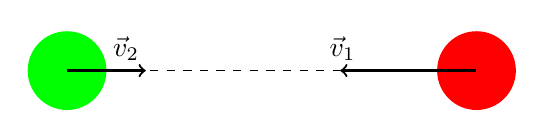
\begin{tikzpicture}
		\draw [dashed] (0,0) -- (5.2,0);
		
		\fill[green] (0,0) circle (0.5cm);
		\fill[red] (5.2,0) circle (0.5cm);
		
		\draw [->, thick] (5.2,0) -- (3.47, 0);
		\node [above] at (3.5, 0) {$\vec{v}_1$};
		
		\draw [->, thick] (0,0) -- (1, 0);
		\node [above] at (0.75,0) {$\vec{v}_2$};
		
		\end{tikzpicture}
		\caption{До задачі \arabic{assigments}.\arabic{problems}}
		
	\end{figure}
\end{problem}

\begin{problem}{2}
	М'яч масою $m = 300$ г впав з висоти $H = 1.23$ м на асфальт і підскочив на ту саму висоту. Удар об асфальт тривав $0.1$ с. Визначте середню силу удару $F_{\text{ср}}$. Як зміниться середня сила удару, якщо м'яч вдариться об тверду поверхню, нахилену під кутом $\alpha = 30^{\circ}$ до горизонту? Якою буде $F_{\text{ср}}$, якщо м'яч замінити кулькою з пластиліну тієї ж маси? Тривалість удару та сама
\end{problem}

\begin{problem}{3}
	Граната, яка летіла зі швидкістю $10~\dfrac{\text{м}}{\text{c}}$, розірвалась на два осколки масами $1.2$ кг та $0.8$ кг. Швидкість більшого осколка досягла $25~\dfrac{\text{м}}{\text{c}}$ за напрямом руху. Яка швидкість меншого осколка?
\end{problem}

\begin{problem}{6}
	Рух матеріальної точки описується рівнянням $x = 5-8t+4t^2$. Вважаючи, що маса точки дорівнює $2$ кг, визначити імпульс через $2$ с і через $4$ с після початку відліку часу а також силу, що викликала зміну імпульсу
\end{problem}

\begin{problem}{11}
	Тіло рівномірно рухається по колу. Модуль його імпульса дорівнює $p$. Визначте модуль зміни імпульса за час, що дорівнює $0.25T$, $0.5T$, $\dfrac{2}{3}T$, T - період обертання.
\end{problem}

\begin{problem}{12}
	Вагон, що має масу $20$ т. рухався зі швидкістю $0.3~\dfrac{\text{м}}{\text{c}}$ і наздогнав вагон, який має масу $30$ т і рухався зі швидкістю $0.2~\dfrac{\text{м}}{\text{c}}$. Яка швидкість вагонів після зчеплення?
\end{problem}

\begin{problem}{14}
	На горизонтальному гладенькому столі вздовж однієї прямої розміщено $2020$ кульок. Маса кожної кульки $m$. Першій кульці надано швидкість $v$. Знайдіть швидкість останньої кульки, якщо всі співужари вбсолюьно пружні.
\end{problem}